%% LyX 2.4.4 created this file.  For more info, see https://www.lyx.org/.
%% Do not edit unless you really know what you are doing.
\documentclass[english]{article}
\usepackage[T1]{fontenc}
\usepackage[latin9]{inputenc}
\usepackage{float}
\usepackage{enumitem}
\usepackage{amsmath}
\usepackage{amsthm}
\usepackage{cancel}
\usepackage{geometry}
\geometry{verbose,tmargin=1in,bmargin=1in,lmargin=1in,rmargin=1in}

\makeatletter

%%%%%%%%%%%%%%%%%%%%%%%%%%%%%% LyX specific LaTeX commands.
%% Because html converters don't know tabularnewline
\providecommand{\tabularnewline}{\\}

%%%%%%%%%%%%%%%%%%%%%%%%%%%%%% Textclass specific LaTeX commands.
\numberwithin{equation}{section}
\numberwithin{figure}{section}
\newlength{\lyxlabelwidth}      % auxiliary length 

%%%%%%%%%%%%%%%%%%%%%%%%%%%%%% User specified LaTeX commands.
\usepackage{hyperref}
\usepackage[usenames,dvipsnames,table]{xcolor} %adds additional color options
\hypersetup{colorlinks=true, urlcolor=black,linkcolor=black}

\usepackage{fancyhdr}
\usepackage{lastpage}
\pagestyle{fancy}
\usepackage{enumitem}
\usepackage{ifthen}
%sets math fonts to be more readable
\everymath=\expandafter{\the\everymath\displaystyle}
%\DeclareMathSizes{10}{10}{10}{10}
\usepackage{multicol}

\usepackage{tikz}
\usetikzlibrary{plotmarks}
\usepackage{pgfplots}
\pgfplotsset{compat=newest}

\usepackage{calc}
\usepackage[nomessages]{fp}

\usepackage{advdate}    % Advancing/saving dates
\usepackage{datetime}   % Dates formatting
\usepackage{datenumber} % Counters for dates

\usepackage{fancybox} %%ovalbox and fancy box settings

\usepackage[super]{nth} %easy 1st, 2nd, etc

\usepackage{forest} %%for tree diagram

%%data for histogram%%
\begin{filecontents}{hist1_data.csv} 
dist 
3
1
0
4
1
3
2
2
0
2
0
2
2
1
4
3
1
1
3
4
2
1
3
0
1
0
2
5
1
2
3
0
0
1
2
3
1
2
0
2
\end{filecontents}

%%data for histogra: cal per cereal%%
\begin{filecontents}{hist_data_cereal.csv} 
dist 
3.7
3.6
3.6
4.0
4.0
3.6
3.8
3.7
4.1
3.9
3.9
3.3
3.5
3.6
3.9
4.0
\end{filecontents}
% Added by lyx2lyx
\setlength{\parskip}{\smallskipamount}
\setlength{\parindent}{0pt}

\makeatother

\usepackage{babel}
\begin{document}
\renewcommand{\author}{Dr.\,James Ashe}

\newcommand{\classNum}{107}

\newcommand{\classSec}{7 and 10}

\newcommand{\nameType}{Name:}

\newcommand{\examType}{Exam 4}

\renewcommand{\date}{ \formatdate{21}{11}{2014}}

%%First page's header%%%%%%%%%%%%%%%%%%%%%%
\fancypagestyle{firststyle} %%header settings for first pagr
{
	\fancyhead[L]{MTH \classNum{}(\classSec{}) \author{}\\
	\textbf{\examType{}} \date{}}
	\fancyhead[C]{\textbf{\nameType}}
	\setlength{\headsep}{14pt}
}
%%%%%%%%%%%%%%%%%%%%%%%%%%%%%%%%%%%%%%%%%%

%%Next page's header%%%%%%%%%%%%%%%%%%%%%%%
%\setlist{nolistsep}
\lhead{MTH \classNum{}(\classSec{})} 
\chead{\textbf{\nameType}} 
\cfoot{\thepage{}~of~\pageref{LastPage}} 
\setlength{\headsep}{5pt} 
%%%%%%%%%%%%%%%%%%%%%%%%%%%%%%%%%%%%%%%%%%%

%%Various settings; see the preamble for other settings%%%%%
%%\setenumerate[0]{leftmargin=12pt,itemindent=0pt,labelwidth=0pt}
%\setlist[2]{noitemsep}
%\setlist{nosep}
\setlist{itemsep=-3pt,topsep=-2pt}
\renewcommand{\labelenumi}{\textbf{\arabic{enumi}.}}
\renewcommand{\labelenumii}{\textbf{\alph{enumii}.}}
\thispagestyle{firststyle}
%%%%%%%%%%%%%%%%%%%%%%%%%%%%%%%%%%%%%%%%%%
\newcommand{\xmax}{10}
\newcommand{\xmin}{-10}
\newcommand{\xstep}{0} %must be xmin+n
\newcommand{\ymax}{10}
\newcommand{\ymin}{-10}
\newcommand{\ystep}{0} %must be ymin+n

\newcommand{\xspace}{\hspace*{40pt}}
\newcommand{\yspace}{\vspace*{1.4cm}}
\newcommand{\rowColor}{gray!35}
\large

\emph{Unless stated otherwise, all problems are worth equal value
and answers should be stated as decimals rounded to three decimal
places. You must show your work to receive credit. }
\begin{enumerate}[resume]
\item Use figure \ref{fig:Number-of-children} to complete the following.\begin{multicols}{2}

\begin{enumerate}
\item Create a frequency distribution table from figure \ref{fig:Number-of-children}
(approximate).

\begin{enumerate}
\item []\Large%
\begin{tabular}{|c|c|}
\hline 
\textbf{hours} & \textbf{freq.}\tabularnewline
\hline 
 & \hspace{0cm}\hphantom{$00$}\tabularnewline
\hline 
 & \tabularnewline
\hline 
 & \tabularnewline
\hline 
 & \tabularnewline
\hline 
 & \tabularnewline
\hline 
\end{tabular}\normalsize\vspace{10pt}
\end{enumerate}
\item Using your frequency table, find the mean.\yspace\vfill
\item What percentage of students are taking less than 14 hours?\vfill\columnbreak
\item []
\begin{figure}[H]
\begin{centering}
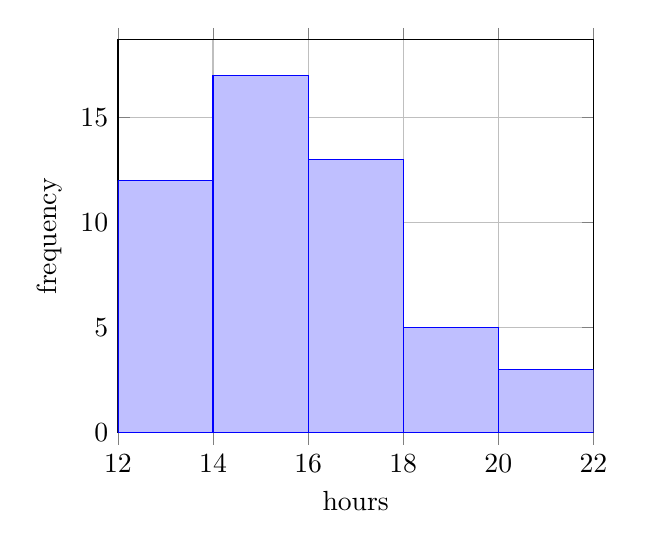
\begin{tikzpicture}[scale=1]
\begin{axis}[     
	ybar interval,
	x tick label as interval=false,    
	ymin=0,
	xmin=12,
	xmax=22,
	width=3in,
	%height=3in,
	grid=major,
	ylabel=frequency,
	xlabel=hours
	] 
	\addplot [fill=blue!25,draw=blue] table [x=Lower, y=Count] { 
		Lower Upper Count 
		12	14	12
		14	16	17
		16	18	13
		18	20	5
		20	22	3
		22	24	0
	};
\end{axis}
\end{tikzpicture}
\par\end{centering}
\caption{\label{fig:Number-of-children}Credit hours of 50 students.}
\end{figure}
\yspace\yspace\yspace
\end{enumerate}
\end{multicols}
\item 10 randomly selected MHU students were surveyed to determine the number
of parking tickets they received this semester. The following results
were found:

\hfill%
\begin{tabular}{cccccccccc}
0 & 7 & 0 & 5 & 1 & 4 & 1 & 2 & 1 & 2\tabularnewline
\end{tabular}\hfill\hspace{0cm}\begin{multicols}{2}
\begin{enumerate}
\item Find the mean.\yspace\yspace
\item Find the median.\yspace
\item Find the mode.\yspace\columnbreak
\item Find the standard deviation.\yspace.\yspace %\begin{tikzpicture}[scale=.8]
%\begin{axis}[     ybar,     ymin=0 ] 
%\addplot +[hist={bins=5,data min=3.2,data max=4.2}] table [y index=0] {hist_data_cereal.csv}; 
%\end{axis} 
%\end{tikzpicture} 
\end{enumerate}
\end{multicols}\newpage
\item Two math 107 sections take an exam, and the following is found. The
\nth{1} section has a mean score of $75$ with standard deviation
$15$, and the \nth{2} section has a mean score of $80$ with a standard
deviation of $10$. 
\item []Are the scores more consistent in the \nth{1} or \nth{2} section?
Why?\vspace{0cm}\vfill
\item A population is normally distributed with mean 50 and standard deviation
15. Draw a sketch of the bell curve labeling the mean and the intervals
representing 1, 2, and 3 standard deviations of the mean.\yspace\yspace\vfill
\item Find the following probabilities,\begin{multicols}{2} 

\begin{enumerate}
\item $p(z<.67)$\yspace\yspace\vfill
\item $p(z>.67)$\yspace\yspace\vfill
\item $p(.09<z<.67)$\yspace\yspace\vfill
\end{enumerate}
\end{multicols}
\item A population is normally distributed with a mean $100$ and standard
deviation $15$. Find the following probabilities. \begin{multicols}{2}

\begin{enumerate}
\item $p(x<75)$\yspace\yspace\vfill
\item $p(75<x<115)$\yspace\yspace\vfill
\end{enumerate}
\end{multicols}\newpage
\item Find $c$ such that each of the following is true.\begin{multicols}{2}

\begin{enumerate}
\item $p(z<c)=9.18\%$\yspace\yspace\yspace\yspace\vfill
\item $p(z>c)=40.95\%$\yspace\yspace\yspace\yspace\vfill
\end{enumerate}
\end{multicols}
\item {[}7 points each{]} The average score on the ACT is $18$ with a standard
deviation of $6$. 

\begin{enumerate}
\item Find the probability that a random test score is below $12$. \yspace\vfill
\item What score separates the \textbf{bottom $48.01\%$ }from the rest
of the population.\yspace\vfill
\end{enumerate}
\newpage
\item {[}BONUS{]} The \emph{Central Limit Theorem }states that for large
enough $n$, then the means of all samples of size $n$ will be normally
distributed. With this in mind, suppose we take a large, randomly
selected sample of men and find that $\bar{x}=70.5$ inches. If it
is known that $\sigma=1.5$ inches, how can we say that this value
is within $3$ inches of the actual mean height, $\mu$, with $95.4\%$
certainty?\vspace*{0cm}\vfill
\end{enumerate}

\section*{Honor Statement}

\emph{On my honor, I have neither given nor received any academic
aid or information that would violate the Honor Code of Mars Hill
University.}\vspace{.5cm}
\begin{itemize}
\item []Signature:\underline{\hspace{7cm}}\vfill
\end{itemize}

\end{document}
